\chapter{Pose Error Estimation}

\section{Introduction}

The main objective of this project is to determine a quadcopter's the pose estimation accuracy, with its pose given by its on-board sensors. Here, the pose refers to a six-dimensional vector describing an object's position and angular orientation. The pose estimation accuracy must be performed in the outdoors to allow the quadcopter to use its global positioning sensor (GPS). To this end, a computer vision pose measurement system (CVS), which extracts six-dimensional pose data from a calibration object in the system's view, was designed and implemented. Before the CVS was used to make pose measurements, its measurement accuracy was first determined. 

In Chapter meme it was found that the pose measurement error of the CVS has high interdimensional dependence, as demonstrated by the covariance matrix of the error and the contour plots in Figure meme, and, despite using the RANSAC algorithm to filter out any outlier data points, the data is still fairly complex and noisy. This means that the measurement error is constantly changing and varies with the calibration board's current pose relative to the CVS's camera.

In the context of this project, it is important to know what the accuracy of a pose measurement sample is to ensure that it is more accurate than the pose estimate from the quadcopter. This makes it necessary to be able to determine the measurement error of any arbitrary pose measurement sample of the CVS.\@ It was decided that machine learning method will be employed to accomplish this. Machine learning is where a computer model is trained to recognise patterns within a set of input data and output information on the patterns which are of interest to the model's designer. 

This chapter sets out to explain the process behind making a machine learning model that can estimate, within reasonable accuracy, what the pose measurement error of the CVS is for any arbitrary input measurement vector. 

\section{Model Design}

\subsection{Background}

Designing a machine learning model can consist of three basic steps. These steps are listed as follows:

\begin{enumerate}
  \item Select machine learning model type.
  \item Train the model.
  \item Validate the model's accuracy. 
\end{enumerate}

First, the model type is selected. As stated previously, the CVS's pose measurement data is fairly complex, interdimensionally dependant and is high dimensional. A neural network model was therefore selected as a basis. It has been shown by~\cite{tu1996advantages} that neural networks excel at handling complex data and detecting and extracting complex non-linear relationships within the input data. Furthermore, the radial basis neural network (RBFNN) was chosen as a neural network topology. RBFNN's provide superior results, when compared to traditional feed-forward networks, when noisy data sets are used, as proven by~\cite{xie2011comparison}. The data is not time dependant, making the recurrent neural network topology unnecessarily complex for this application.  

Next, model training takes place. Here, the network is trained to take an input and adjust is internal weights in such a way that the input data is best related to a desired output by using a supervised training scheme, such as the backpropagation procedure. In this case, the network input would be the six-dimensional pose vector produced by the CVS and the network output is the corresponding measurement error of the input pose vectors.  

Finally, to test and validate the accuracy of the trained model, it is tested with another set of input pose data of which the measurement error is already known. These two data sets can be used to select and refine the training parameters of the model. 

The design process is iterative, where steps 2 and 3, and perhaps 1, can be repeated until a model which outputs satisfactory results is produced. 

\subsection{Model Training}

Training a machine learning model is perhaps the most crucial aspect of the model design phase. Here the hidden layer of the RBFNN's nodes are initialised and assigned a weighting factor. This weight is selected in such a way that it minimises the difference between the network's output and the training error data by using the backpropagation method, demonstrated in Figure~\ref{fig:chap4-backprogagation}.

\begin{figure}
  \centering
  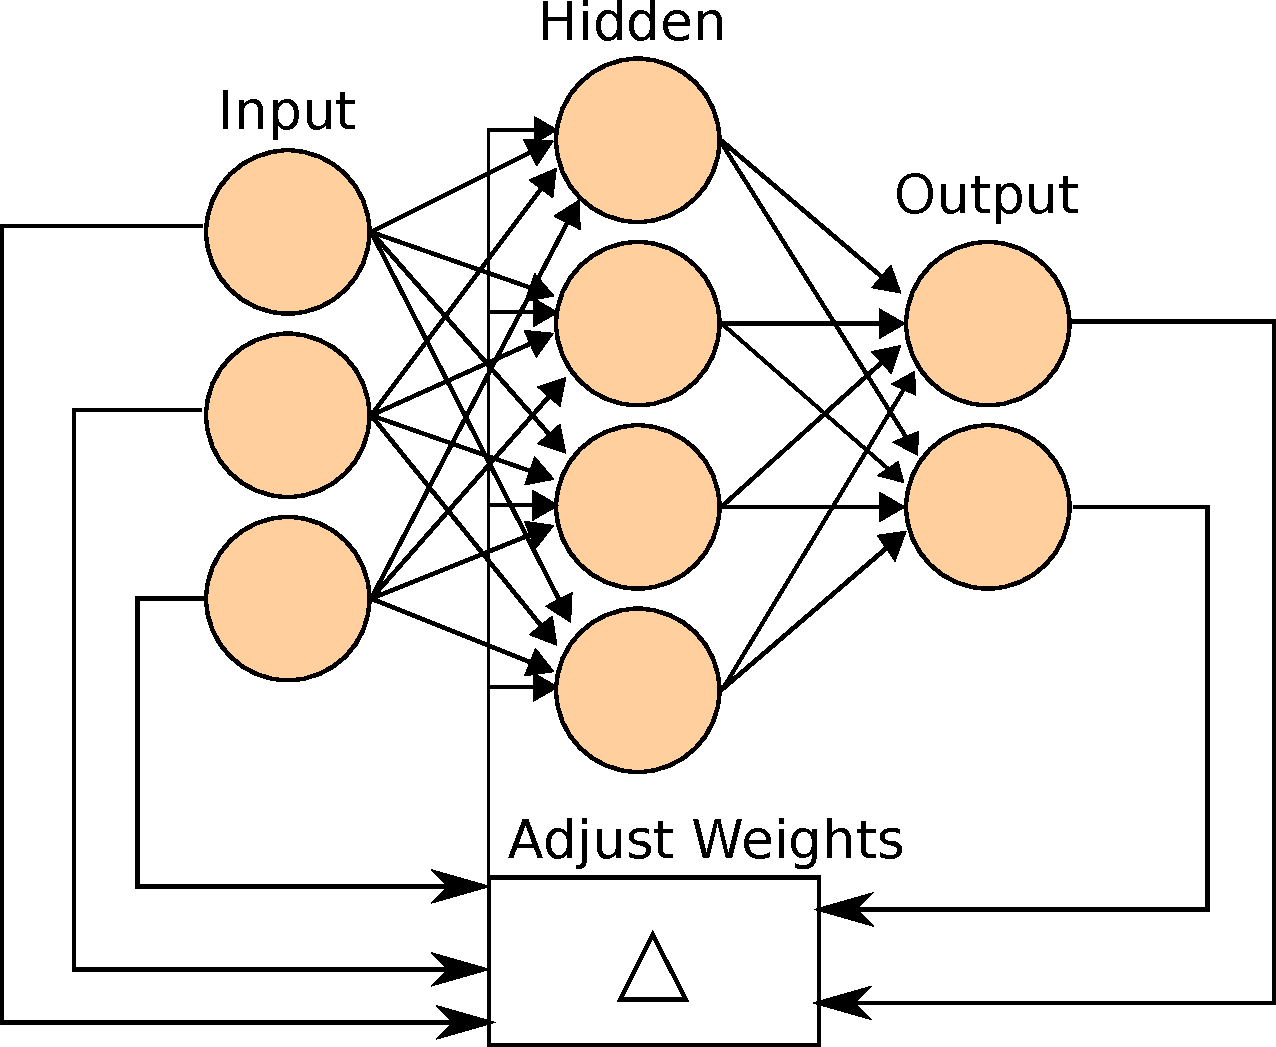
\includegraphics[width=0.5\textwidth]{figures/chapter4/backpropagation}
  \caption[A neural network implementing the backpropagation procedure.]{A figure of a neural network implementing the backpropagation procedure. Adopted from~\cite{ann-wiki-pic}.}
\label{fig:chap4-backprogagation}
\end{figure}

The backpropagation method works as follows. The hidden nodes are initialised with a weighting factor. The input training data is then fed to the network and the output is compared to the training set's output data. Based on this difference, the different nodes' weighting factors are adjusted. Then, the input data is fed to the adjusted network again and the new output is compared to the output training data. This process is repeated until the mean square error of the output's deviation from the training data falls below a set threshold. 

Factors that will affect the network's accuracy are the number of nodes in the hidden layer, as well as the strictness of fit. The number of hidden nodes is a measure of the complexity of the network and reflects the complexity of the data it can process. However, when too many nodes are selected, there is a significant risk that the model will only capture and attempt to model the noise and outlier data in a data set, instead of characterising the underlying relationships between the input and output. This phenomenon is known as overfitting and can be observed when a model with a very small training error is exposed to new input data and the error is a few orders of magnitude larger than for the training data. Here, the model describes the training data set very well, but any data set that is not very similar to the training data set will be handled very poorly. This is why the model validation phase is a very important aspect of model training, to ensure that overfitting does not take place. 

To train the model for this project, two sets of data were used, one for training and another for the model validation. Both of these data sets were taken from the data sets generated during the Vicon measurement test, where the measurement accuracy of the CVS was determined by comparing its measurements to that of the measurements made by a Vicon system. It includes both the pose data from the CVS and the corresponding measurement error. It was decided to use 300 training samples, giving 50 samples per dimension. The input and output training data sets were normalised to a range of $[-1, 1]$, since the pose vector contains different measurement units (degrees and metres). All subsequent inputs to and outputs from the network must be normalised and denormalised with the same values that the training data was normalised with.  

Matlab's\footnote{Matlab v8.4.0.150421 (R2014)} Neural Network toolbox\footnote{Neural Network Toolbox v8.2.1} was used to train the RBFNN and get the output for subsequent input data. The function prototype is given by 

\begin{center}
  \verb|net = newrb(P,T,goal,spread,MN,DF)|
\end{center}

Here, $P$ and $T$ are the $300\times6$ input and output training data matrices. The `goal' parameter is the error threshold for the training data and `spread' is the strictness of fit parameter, while $MN$ and $DF$ define the maximum number of hidden nodes and dictate the amount of nodes to increase by between each training iteration. Adjusting the `spread' and $MN$ parameters are the primary ways of adjusting the network's accuracy and output. 

\subsection{Model Validation}

The model validation phase is used to ensure that the RBFNN has been properly trained and that overfitting does not occur. The validation data set comes from the same Vicon test the training data comes from. Another 300 pose measurement samples were used for the validation data set. 

The error was determined by feeding the validation input data into the trained network and comparing its output with the validation error data. The mean square error was used as a measure of accuracy. 

\section{Results}

With the training and validation data sets selected, the model design could begin. Different combinations of training parameters for the `newrb' Matlab function were tested. It was found that the `spread' parameter played the largest part in the mean square error during training. This is because the training data changes relatively quickly and contains a fair amount of noise. It was found that forcing the RBFNN to go through all the points caused the mean square error to go up when it was tested with the validation set. It was therefore decided to keep the spread parameter small to allow the RBFNN to describe the general trend in the data. 

Furthermore, changing the maximum number of nodes also influenced the accuracy of the network. Leaving the $MN$ parameter to its default will let the maximum number of hidden nodes go up to the number of training samples, i.e.\ 300 nodes in this case. This makes the network overly complex and slow. It was found that the network performs better with both the training and validation data sets with a lower number of nodes, at about 10\% of the number of samples. 

A combination that was found to work well, was a `spread' of 1\e{-3} and 20 hidden nodes. This combination gives a mean square error of approximately 3.0, whereas the default values of 1 and 300 gives a mean square error of 5\e{3} meme bewys, indicating a significant improvement in accuracy. SIT IN TRAINING AND VALIDATION GRAFIEKE. BESPREEK AKKURAATHEID VAN AFSKATTINGS.  

Figure~\ref{fig:chap4-rbf-train} shows results of the RBFNN model when tested with the training data set. It can be seen that the model's estimate very closely resembles the training set's error, indicating that the model is well-trained. 

\begin{figure*}
  \begin{subfigure}{0.3\textwidth}
    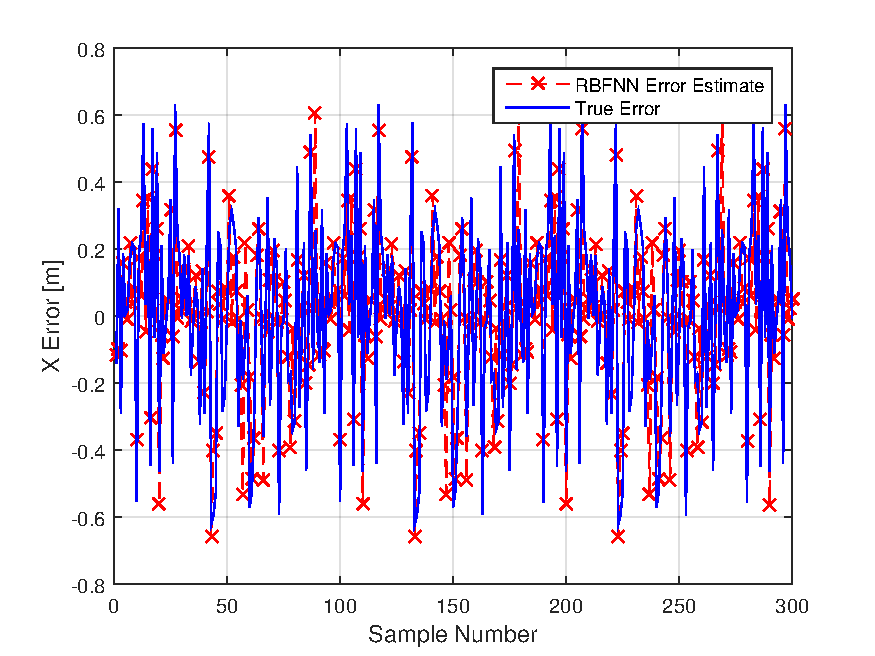
\includegraphics[width=\textwidth]{figures/chapter4/x_train}
    \caption{}
  \end{subfigure}
~
  \begin{subfigure}{0.3\textwidth}
    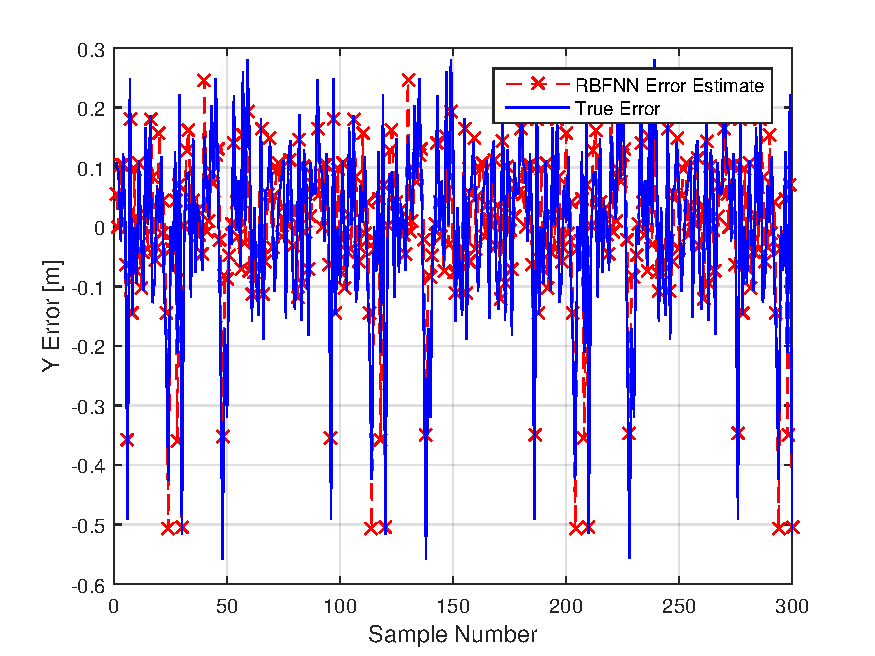
\includegraphics[width=\textwidth]{figures/chapter4/y_train}
    \caption{}
  \end{subfigure}
~
  \begin{subfigure}{0.3\textwidth}
    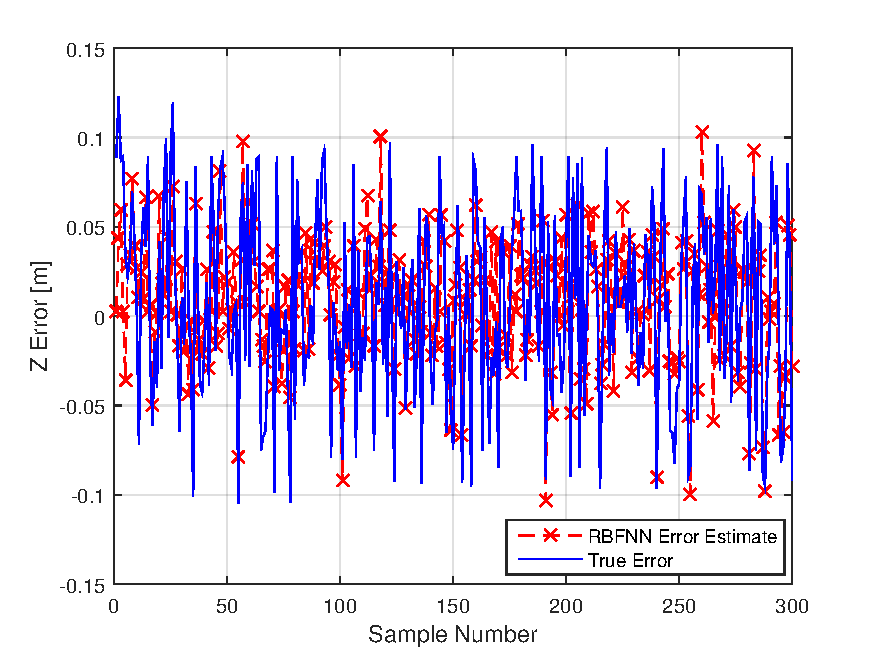
\includegraphics[width=\textwidth]{figures/chapter4/z_train}
    \caption{}
  \end{subfigure}
~
  \begin{subfigure}{0.3\textwidth}
    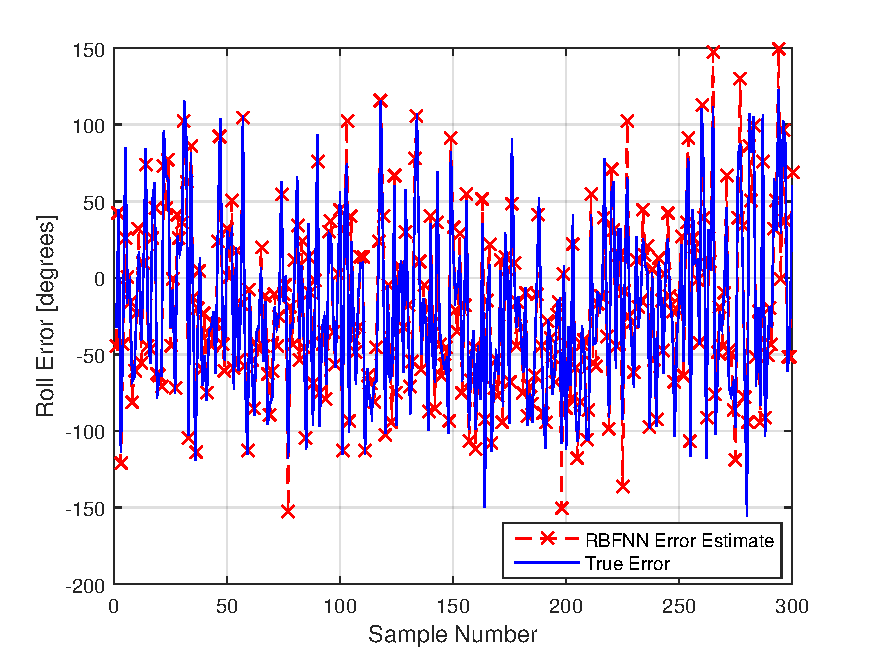
\includegraphics[width=\textwidth]{figures/chapter4/roll_train}
    \caption{}
  \end{subfigure}
~
  \begin{subfigure}{0.3\textwidth}
    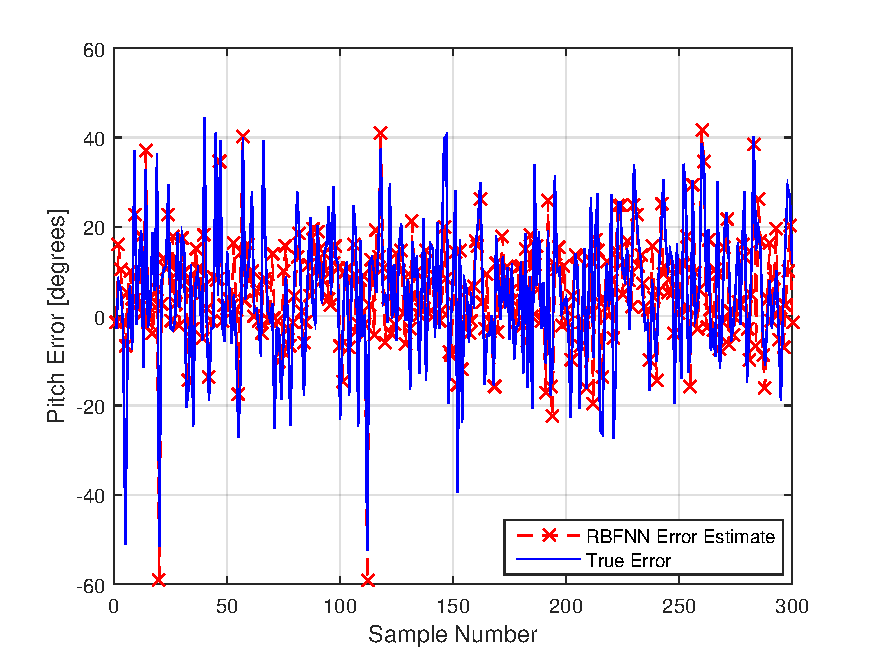
\includegraphics[width=\textwidth]{figures/chapter4/pitch_train}
    \caption{}
  \end{subfigure}
~
  \begin{subfigure}{0.3\textwidth}
    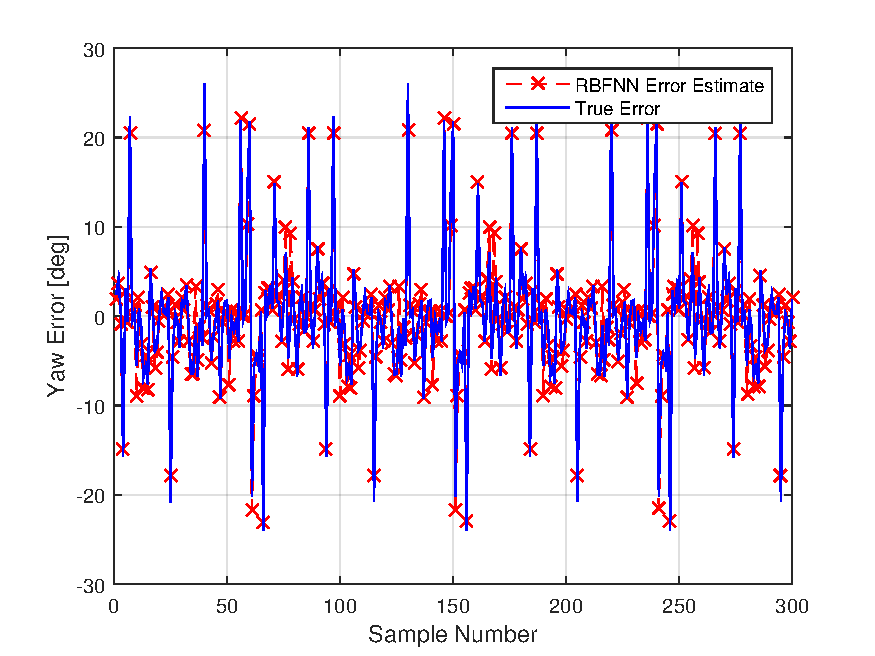
\includegraphics[width=\textwidth]{figures/chapter4/yaw_train}
    \caption{}
  \end{subfigure}
  \caption[The output of the RBFNN when used with the training set input.]{A plot of the output of the RBFNN for the different dimensions when used with the training data set.}
  \label{fig:chap4-rbf-train}
\end{figure*}

Figure~\ref{fig:chap4-rbf-valid} shows the model's output when tested with the validation data set.

\begin{figure*}
  \begin{subfigure}{0.3\textwidth}
    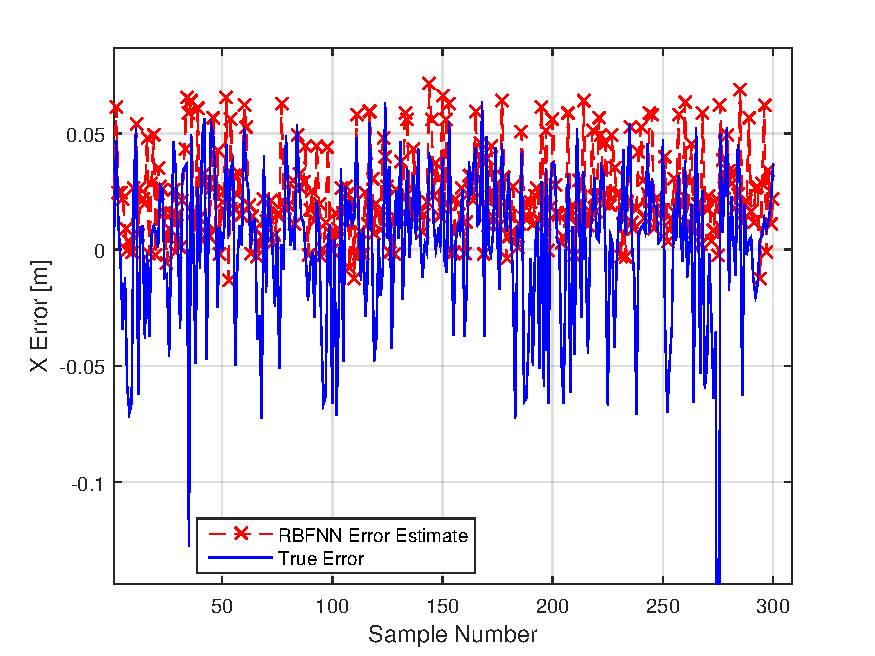
\includegraphics[width=\textwidth]{figures/chapter4/x_valid}
    \caption{}
  \end{subfigure}
~
  \begin{subfigure}{0.3\textwidth}
    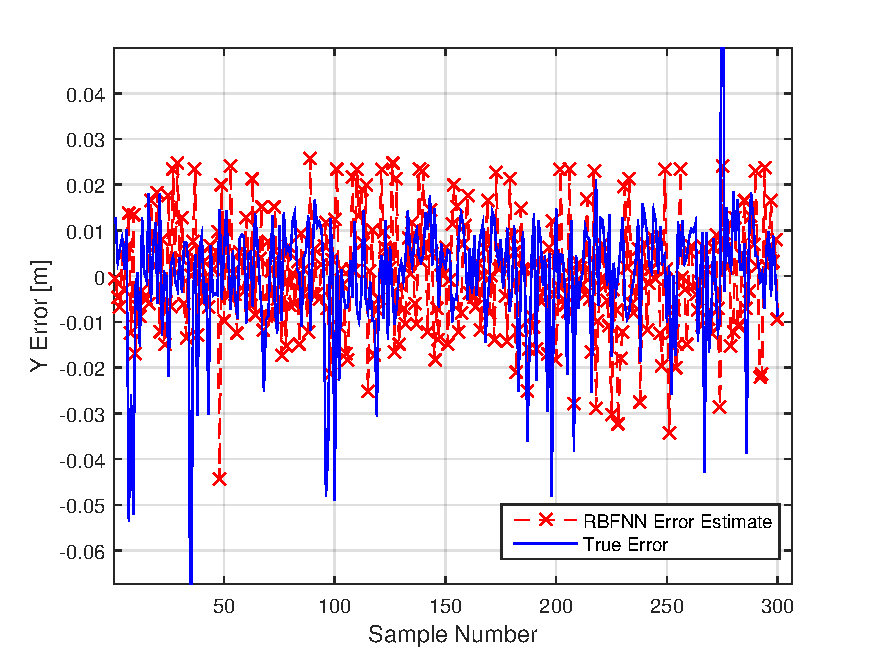
\includegraphics[width=\textwidth]{figures/chapter4/y_valid}
    \caption{}
  \end{subfigure}
~
  \begin{subfigure}{0.3\textwidth}
    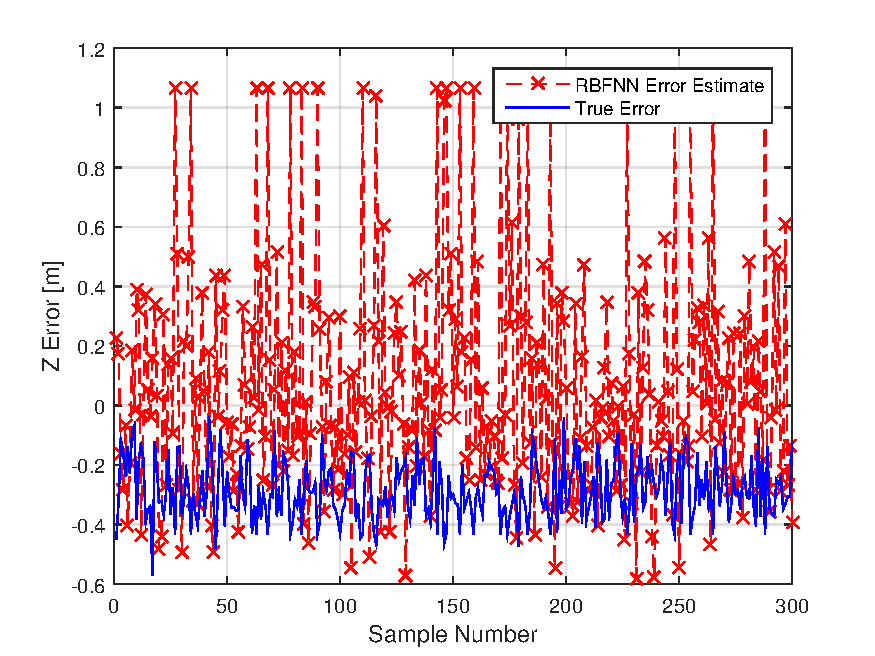
\includegraphics[width=\textwidth]{figures/chapter4/z_valid}
    \caption{}
  \end{subfigure}
~
  \begin{subfigure}{0.3\textwidth}
    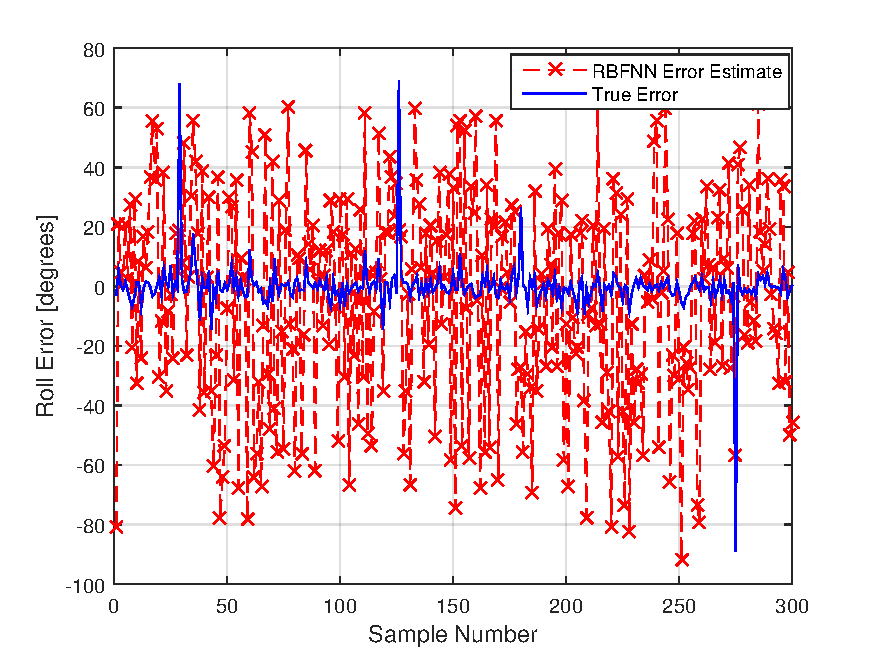
\includegraphics[width=\textwidth]{figures/chapter4/roll_valid}
    \caption{}
  \end{subfigure}
~
  \begin{subfigure}{0.3\textwidth}
    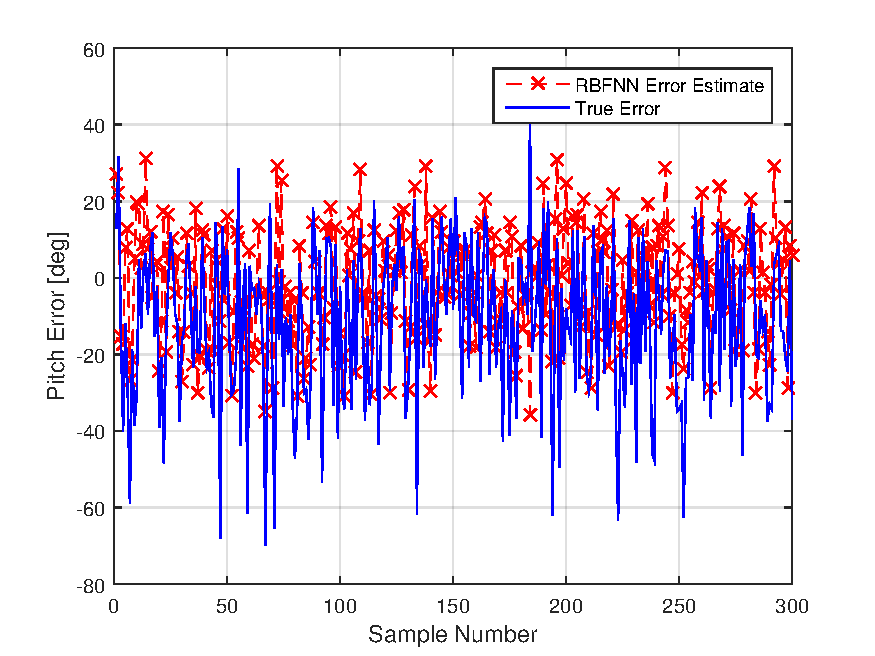
\includegraphics[width=\textwidth]{figures/chapter4/pitch_valid}
    \caption{}
  \end{subfigure}
~
  \begin{subfigure}{0.3\textwidth}
    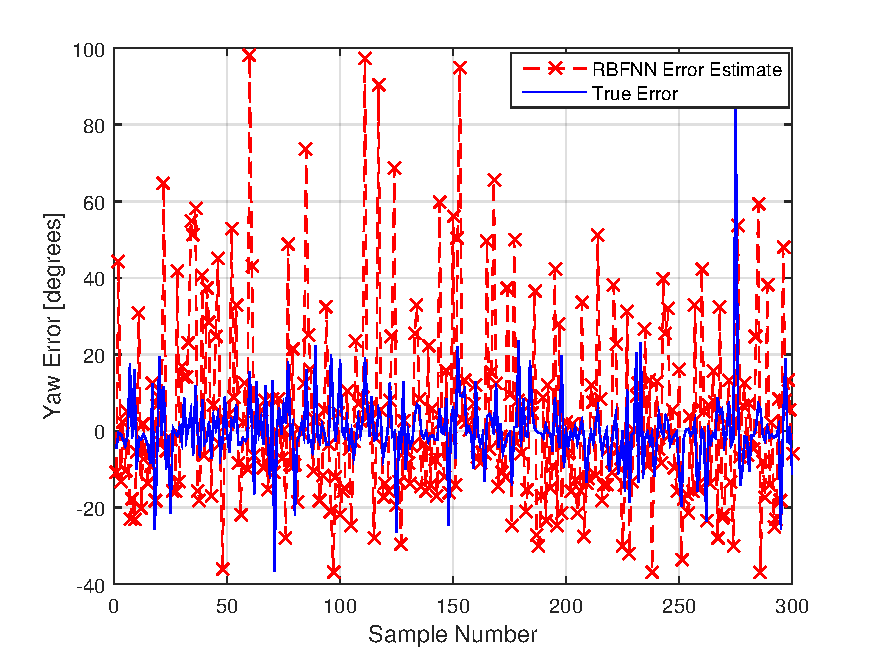
\includegraphics[width=\textwidth]{figures/chapter4/yaw_valid}
    \caption{}
  \end{subfigure}
  \caption[The output of the RBFNN with the validation set input.]{A plot of the output for the different dimensions of the RBFNN when used with the validation data set.}
  \label{fig:chap4-rbf-valid}
\end{figure*}

\section{Conclusion}

In this chapter, a machine learning model was designed to model and predict the complex and dimensionally dependant error data of the CVS.\@ A radial basis function neural network was selected to do this: it takes a six-dimensional pose measurement vector from the CVS and outputs the corresponding measurement error for the input sample. The network was trained and validated by two different data sets from the same measurement test and produces a mean square error of 3.0 for the validation set, indicating a good fit. 

The trained network is now ready to predict the measurement error for the CVS with pose measurement data generated by a quadcopter in flight. This data can then be used to determine the pose estimation accuracy of a drone in flight. 

